%----------------------------------------------------------------------------------------
%	PACKAGES AND OTHER DOCUMENT CONFIGURATIONS
%----------------------------------------------------------------------------------------
\documentclass[11pt,a4paper,italian,twoside,twocolumn]{article}
\pagenumbering{arabic}
\usepackage{setspace}
%\onehalfspace
\usepackage[hmarginratio=1:1,top=32mm,columnsep=20pt]{geometry}
\usepackage{fancyhdr}
\usepackage{multirow}
\usepackage{multicol}
\usepackage[section]{placeins}
%--Text and Style------------------------------------------------------------------------
\usepackage{microtype} 			% Slightly tweak font spacing for aesthetics
\usepackage[italian]{babel} 		% Language hyphenation and typographical rules
\usepackage[T1]{fontenc}
\usepackage[utf8]{inputenc}
\usepackage{ae}
\usepackage{relsize}
\usepackage{csquotes} 
\usepackage{amsmath}
\usepackage{amsfonts}
\usepackage{mathdots}
\usepackage{mathtools}
\usepackage[colorlinks=true]{hyperref}
\hypersetup{
	bookmarksnumbered=true,
	linkcolor=black,
	citecolor=black,
	%pagecolor=black,
	urlcolor=black,
}
\usepackage{verbatim}
\usepackage{alltt}
\DeclareMathOperator{\sgn}{sgn}
\DeclareMathOperator{\RealNumber}{\rm I\!R}
\DeclarePairedDelimiter{\abs}{\lvert}{\rvert}
\DeclarePairedDelimiter{\norma}{\lVert}{\rVert}
\usepackage{lipsum}
\usepackage{siunitx}
\usepackage[inline]{enumitem}
\usepackage{lettrine}

%---Figure------------------------------------------------------------------------------

\usepackage{graphicx}
\graphicspath{{./imgs/}}
\renewcommand{\figurename}{Fig.}
\usepackage{subfig}

%---------------------------------------------------------------------------------------
\usepackage{algorithmicx}
\usepackage[ruled]{algorithm}
\usepackage{algpseudocode}
\usepackage{listings}
\usepackage{xcolor}
\definecolor{halfgray}{gray}{0.55}
\definecolor{ipython_frame}{RGB}{207, 207, 207}
\definecolor{ipython_bg}{RGB}{247, 247, 247}
\definecolor{ipython_red}{RGB}{186, 33, 33}
\definecolor{ipython_green}{RGB}{0, 128, 0}
\definecolor{ipython_cyan}{RGB}{64, 128, 128}
\definecolor{ipython_purple}{RGB}{170, 34, 255}
\lstset{
    breaklines=true,
    %
    extendedchars=true,
    literate=
    {á}{{\'a}}1 {é}{{\'e}}1 {í}{{\'i}}1 {ó}{{\'o}}1 {ú}{{\'u}}1
    {Á}{{\'A}}1 {É}{{\'E}}1 {Í}{{\'I}}1 {Ó}{{\'O}}1 {Ú}{{\'U}}1
    {à}{{\`a}}1 {è}{{\`e}}1 {ì}{{\`i}}1 {ò}{{\`o}}1 {ù}{{\`u}}1
    {À}{{\`A}}1 {È}{{\'E}}1 {Ì}{{\`I}}1 {Ò}{{\`O}}1 {Ù}{{\`U}}1
    {ä}{{\"a}}1 {ë}{{\"e}}1 {ï}{{\"i}}1 {ö}{{\"o}}1 {ü}{{\"u}}1
    {Ä}{{\"A}}1 {Ë}{{\"E}}1 {Ï}{{\"I}}1 {Ö}{{\"O}}1 {Ü}{{\"U}}1
    {â}{{\^a}}1 {ê}{{\^e}}1 {î}{{\^i}}1 {ô}{{\^o}}1 {û}{{\^u}}1
    {Â}{{\^A}}1 {Ê}{{\^E}}1 {Î}{{\^I}}1 {Ô}{{\^O}}1 {Û}{{\^U}}1
    {œ}{{\oe}}1 {Œ}{{\OE}}1 {æ}{{\ae}}1 {Æ}{{\AE}}1 {ß}{{\ss}}1
    {ç}{{\c c}}1 {Ç}{{\c C}}1 {ø}{{\o}}1 {å}{{\r a}}1 {Å}{{\r A}}1
    {€}{{\EUR}}1 {£}{{\pounds}}1
}

%%
%% Python definition (c) 1998 Michael Weber
%% Additional definitions (2013) Alexis Dimitriadis
%% modified by me (should not have empty lines)
%%
\lstdefinelanguage{iPython}{
    morekeywords={access,and,break,class,continue,def,del,elif,else,except,exec,finally,for,from,global,if,import,in,is,lambda,not,or,pass,print,raise,return,try,while},%
    %
    % Built-ins
    morekeywords=[2]{abs,all,any,basestring,bin,bool,bytearray,callable,chr,classmethod,cmp,compile,complex,delattr,dict,dir,divmod,enumerate,eval,execfile,file,filter,float,format,frozenset,getattr,globals,hasattr,hash,help,hex,id,input,int,isinstance,issubclass,iter,len,list,locals,long,map,max,memoryview,min,next,object,oct,open,ord,pow,property,range,raw_input,reduce,reload,repr,reversed,round,set,setattr,slice,sorted,staticmethod,str,sum,super,tuple,type,unichr,unicode,vars,xrange,zip,apply,buffer,coerce,intern},%
    %
    sensitive=true,%
    morecomment=[l]\#,%
    morestring=[b]',%
    morestring=[b]",%
    %
    morestring=[s]{'''}{'''},% used for documentation text (mulitiline strings)
    morestring=[s]{"""}{"""},% added by Philipp Matthias Hahn
    %
    morestring=[s]{r'}{'},% `raw' strings
    morestring=[s]{r"}{"},%
    morestring=[s]{r'''}{'''},%
    morestring=[s]{r"""}{"""},%
    morestring=[s]{u'}{'},% unicode strings
    morestring=[s]{u"}{"},%
    morestring=[s]{u'''}{'''},%
    morestring=[s]{u"""}{"""},%
    %
    % {replace}{replacement}{lenght of replace}
    % *{-}{-}{1} will not replace in comments and so on
    literate=
    *{+}{{{\color{ipython_purple}+}}}1
    {-}{{{\color{ipython_purple}-}}}1
    {*}{{{\color{ipython_purple}$^\ast$}}}1
    {/}{{{\color{ipython_purple}/}}}1
    {^}{{{\color{ipython_purple}\^{}}}}1
    {?}{{{\color{ipython_purple}?}}}1
    {!}{{{\color{ipython_purple}!}}}1
    {\%}{{{\color{ipython_purple}\%}}}1
    {<}{{{\color{ipython_purple}<}}}1
    {>}{{{\color{ipython_purple}>}}}1
    {|}{{{\color{ipython_purple}|}}}1
    {\&}{{{\color{ipython_purple}\&}}}1
    {~}{{{\color{ipython_purple}~}}}1
    %
    {==}{{{\color{ipython_purple}==}}}2
    {<=}{{{\color{ipython_purple}<=}}}2
    {>=}{{{\color{ipython_purple}>=}}}2
    %
    {+=}{{{+=}}}2
    {-=}{{{-=}}}2
    {*=}{{{$^\ast$=}}}2
    {/=}{{{/=}}}2,
    %
    literate=
    {á}{{\'a}}1 {é}{{\'e}}1 {í}{{\'i}}1 {ó}{{\'o}}1 {ú}{{\'u}}1
    {Á}{{\'A}}1 {É}{{\'E}}1 {Í}{{\'I}}1 {Ó}{{\'O}}1 {Ú}{{\'U}}1
    {à}{{\`a}}1 {è}{{\`e}}1 {ì}{{\`i}}1 {ò}{{\`o}}1 {ù}{{\`u}}1
    {À}{{\`A}}1 {È}{{\'E}}1 {Ì}{{\`I}}1 {Ò}{{\`O}}1 {Ù}{{\`U}}1
    {ä}{{\"a}}1 {ë}{{\"e}}1 {ï}{{\"i}}1 {ö}{{\"o}}1 {ü}{{\"u}}1
    {Ä}{{\"A}}1 {Ë}{{\"E}}1 {Ï}{{\"I}}1 {Ö}{{\"O}}1 {Ü}{{\"U}}1
    {â}{{\^a}}1 {ê}{{\^e}}1 {î}{{\^i}}1 {ô}{{\^o}}1 {û}{{\^u}}1
    {Â}{{\^A}}1 {Ê}{{\^E}}1 {Î}{{\^I}}1 {Ô}{{\^O}}1 {Û}{{\^U}}1
    {œ}{{\oe}}1 {Œ}{{\OE}}1 {æ}{{\ae}}1 {Æ}{{\AE}}1 {ß}{{\ss}}1
    {ç}{{\c c}}1 {Ç}{{\c C}}1 {ø}{{\o}}1 {å}{{\r a}}1 {Å}{{\r A}}1
    {€}{{\EUR}}1 {£}{{\pounds}}1,
    %
%   identifierstyle=\color{red}\ttfamily,
    commentstyle=\color{ipython_cyan}\ttfamily,
    stringstyle=\color{ipython_red}\ttfamily,
    keepspaces=true,
    showspaces=false,
    showstringspaces=false,
    %
    rulecolor=\color{ipython_frame},
    frame=single,
    frameround={t}{t}{t}{t},
    framexleftmargin=6mm,
    numbers=left,
    numberstyle=\tiny\color{halfgray},
    %
    %
    backgroundcolor=\color{ipython_bg},
    %   extendedchars=true,
    basicstyle=\scriptsize\ttfamily,
    keywordstyle=\color{ipython_green}\ttfamily,
}

%------Matlab scheme color-code----------------------------------
\usepackage{matlab-prettifier}
\lstset{
	style = Matlab-editor,
	basicstyle=\mlttfamily,
    %Style frame and number
    rulecolor = \color{ipython_frame},
    frame	=single,
    frameround={t}{t}{t}{t},
    framexleftmargin=6mm,
    numbers=left,
    numberstyle=\tiny\color{halfgray},
	%background color frame
    backgroundcolor=\color{ipython_bg}   
}

%---Table------------------------------------------------------------
\usepackage{tabularx}
\usepackage{array}
\usepackage{color}
\usepackage{adjustbox}
\usepackage{colortbl}
\usepackage{pgfplotstable}
\usepackage{makecell}
\usepackage{booktabs}

%--------------------------------------------------------------------
% Allows abstract customization
\usepackage{abstract}
% Set the "Abstract" text to bold
\renewcommand{\abstractnamefont}{\normalfont\bfseries} 
% Set the abstract itself to small italic text
\renewcommand{\abstracttextfont}{\normalfont\small\itshape} 
% Allows customization of titles
\usepackage{titlesec} 
% Roman numerals for the sections
\renewcommand\thesection{\Roman{section}} 
% roman numerals for subsections
\renewcommand\thesubsection{\roman{subsection}} 
% Change the look of the section titles
\titleformat{\section}[block]{\large\scshape\centering}{\thesection.}{1em}{} 
% Change the look of the section titles
\titleformat{\subsection}[block]{\large}{\thesubsection.}{1em}{} 
\usepackage{titling} % Customizing the title section

%----------------------------------------------------------------------------------------
\usepackage{tikz,fp,ifthen,fullpage}
\usepackage{pgfmath, pgfplots, xparse}
\usepgfplotslibrary{fillbetween}
\usetikzlibrary{backgrounds, arrows}
\usetikzlibrary{decorations.pathmorphing,fit,through}
\usetikzlibrary{shapes,decorations,shadows}
\usetikzlibrary{fadings,patterns,mindmap}
\usepackage{tikz-dimline, calc}
\pgfplotsset{compat=newest}

%----------------------------------------------------------------------------------------
%	TITLE SECTION
%----------------------------------------------------------------------------------------
\setlength{\droptitle}{-4\baselineskip} % Move the title up
\pretitle{\begin{center}\Huge\bfseries} % Article title formatting
\posttitle{\end{center}} % Article title closing formatting
\title{TITOLO DA INSERIRE} % Article title %TODO scegliere e inserire titolo
\author{%
	\textsc{Francesco Argentieri}\thanks{ID: 183892}\\[1ex] % Your name
	\normalsize Università di Trento \\ % Your institution
	% Your email address
	\normalsize \href{mailto:francesco.argentieri@studenti.unitn.it}{francesco.argentieri@studenti.unitn.it}%
%% Uncomment if 2 authors are required, duplicate these 4 lines if more
\and 
\textsc{Giacomo Mazzaglia}\thanks{ID: 183382} \\[1ex] % Second author's name 
\normalsize Università di Trento \\ % Second author's institution
\normalsize \href{mailto:giacomo.mazzaglia@studenti.unitn.it}{giacomo.mazzaglia@studenti.unitn.it}%
}
%\date{} % Leave empty to omit a date
\renewcommand{\maketitlehookd}{\begin{abstract}
In questo lavoro, consideriamo il problema di esplorare un ambiente sconosciuto con un team di robot. Come nell'esplorazione di robot singoli, l'obiettivo è di ridurre al minimo il tempo di esplorazione complessivo. Il problema chiave da risolvere nel contesto di robot multipli è quello di scegliere i punti di destinazione appropriati per i singoli robot in modo che possano esplorare contemporaneamente diverse regioni dell'ambiente. Presentiamo un approccio per il coordinamento di più robot, che tiene conto simultaneamente del costo di raggiungere un punto target e della sua utilità. Ogni volta che un punto target viene assegnato a un robot specifico, l'utilità dell'area inesplorata visibile da questa posizione target viene ridotta. In questo modo, le diverse posizioni di destinazione vengono assegnate ai singoli robot. Descriviamo inoltre come il nostro algoritmo può essere esteso a situazioni in cui il raggio di comunicazione dei robot è limitato.Per la stima delle posizioni dei robot è stato utilizzato il filtro particellare,assumendo una comunicazione con delle ancore wi-fi. I risultati dimostrano che la nostra tecnica distribuisce efficacemente i robot sull'ambiente e consente loro di compiere rapidamente la loro missione.
\end{abstract}
} %TODO modificare abstract nel file
%----------------------------------------------------------------------------------------
\begin{document}
	% Print the title
	\maketitle	
	%Other chapter
	\clearpage
	\newpage
% Sommario Introduzione
	\section{Introduzione}
L'esplorazione efficiente di ambienti sconosciuti è un problema fondamentale nella robotica mobile. 
L'estensione alla esplorazione di più robot pone diverse nuove sfide, tra cui: coordinamento di robot , integrazione delle informazioni raccolte dai robot in una mappa coerente; e comunicazione limitata.
Il coordinamento di un sistema di più robot è la base per un'efficiente implementazione di una esplorazione distribuita. Difficoltà maggiore nel campo del coordinamento vengono dalle conoscenze che si assumono avere i robot sul comportamento degli altri robot. Se i robot conoscono le loro posizioni relative e condividono una mappa della zona che hanno esplorato finora, si può raggiungere un coordinamento efficace, guidando i robot in zone inesplorate dell'ambiente.
Questo può essere fatto assegnando ai robot il compito di raggiungere un loro punto di arrivo preso dalla frontiera fornita dalla scansione del lidar(paper).Per un assegnamento efficace è importante che i robot quando vadano a condividere dei punti comuni all'interno delle loro frontiere che non cerchino di raggiungere lo stesso punto.
Per la stima della posizione viene adottato un filtro particellare, i robot comunicando con delle ancore wi-fi riescono a conoscere con un dato errore la loro posizione ricoperta in quell'istante. Per il raggiungimento della zona target prefissata viene invece adottata la funzione potenziale.
I robot contengono al loro interno memoria delle zone già esplorate e non, ipotizzando di conoscere in anticipo le dimensioni massime della mappa che andranno ad eslporare quest'ultimi costruiscono attraverso l'integrazione di successive matrici di occupazione locale una matrice di occupazione globale che rappresenta la mappatura dell'ambiente.
Saranno successivamente presentati la modellazione del sistema e i successivi risultati ottenuti



% Comunicazione
    \section{Comunicazione}
All'interno del sistema realizzato i robot sono in comunicazione tramite rete 
\textsc{Wi-Fi} ideale senza degradazione di segnale e conseguente perdita di 
informazione.
Il primo tipo di comunicazione è quella disponibile tra robot che permette in 
un range limitato l'assegnazione e la coordinazione efficiente della 
destinazione per lo svolgimento della missione.
La seconda tipologia di comunicazione riguarda la stima della posizione dei 
robot mediante \emph{particle filter} per la localizzazione rispetto hotspot 
\textsc{Wi-Fi} intesi, in questo caso, come punti di riferimento virtuali.
Generati casualmente o tramite input dell'utente all'interno 
della mappa.
    
% Modello sistema	
	\section{Modello del sistema}
\subsection{Modello cinematico}
Il robot è basato sul modello dell'uniciclo a trazione differenziale, la configurazione è completamente descritta da $\mathbf{q} = [x \, y \, \theta]^T$, dove $(x,y)$ sono le coordinate cartesiane del punto di contatto con il suolo e $\theta$ è l'orientamento della ruota rispetto l'asse $x$.\cite{siciliano2008robotica}, come in figura \ref{fig:model}.
Il modello cinematico dell'uniciclo è descritto dall'equazioni (\ref{eq:modelcinematico}):
\begin{equation}
\label{eq:modelcinematico}
	\begin{bmatrix}
		\dot{x} \\ 
		\dot{y} \\ 
		\dot{\theta}
	\end{bmatrix} = 
	\begin{bmatrix}
		\cos \theta \\
		\sin \theta \\
		0
	\end{bmatrix} \, v + 
	\begin{bmatrix}
		0 \\
		0 \\
		1
	\end{bmatrix} \, \omega
\end{equation}
\begin{table}[htb]
	\centering
	\caption{Riepilogo dimensioni}
	\label{tab:dimensrobot}
	\begin{tabular}{lcS[table-format=3.2]}
	\toprule
	\multicolumn{3}{c}{dimensioni}\\
	\midrule
      raggio ruote  & [\si{\metre}] & 0.07\\ % dimension wheel [m]
      interasse     & [\si{\metre}] & 0.30\\ % dimension interaxle [m]
     \bottomrule
\end{tabular}
\end{table}
Il robot ha le dimensioni riportate in tabella \ref{tab:dimensrobot}.
Questo è equipaggiato con un sensore virtuale \emph{lidar}, basato sul modello Hokuyo URG-04LX, collocato al centro della struttura in modo tale da evitare errori di offset, di seguito se ne riportano le caratteristiche, di cui adattate ad hoc per la simulazione. Come sensori propriocettivi presenta due encoder incrementali virtuali calettati sull'asse delle ruote, le caratteristiche di entrambi sono riportate in tabella \ref{tab:sensordata}. Una rappresentazione del robot è osservabile in figura \ref{fig:model}.
\begin{table}[htb]
	\centering
	\caption{Specifiche sensori}
	\label{tab:sensordata}
	\begin{tabular}{lcS[table-format=3.2]}
	\toprule
	\multicolumn{3}{c}{specifiche lidar virtuale}\\
	\midrule
 		risoluzione angolare & [\si{\degree}]	& 0.36\\  % [deg] laser sensor parameters\\
 		angolo di scansione  & [\si{\degree}]	& 180.00\\
 		massima distanza		 & [\si{\metre}]		& 4.00	\\ % [m] laser sensor parameters Max FOV
 		minima distanza 		 & [\si{\metre}]		& 0.02	\\ % [m] laser sensor parameters min FOV
 		risoluzione 			 & [\si{\milli\metre}]& 1.00\\
%        % noise
%        laser_rho_sigma     = 0.02;             % variance
%        laser_theta_sigma   = 0.1 * (pi / 180); % variance
	\bottomrule
	\multicolumn{3}{c}{specifiche encoder virtuale}\\
	\midrule
	 risoluzione &  $2 \cdot (\frac{\pi}{2600})$\\   % encoder quantization
        % encoder noise
        %enc_mu = 0;                           % mean
        %enc_sigma = 2 * (2 * pi / 2600) / 3;  % variance
	\bottomrule
	\end{tabular}
\end{table}
%\clearpage
%\onecolumn
\begin{figure}[!h]
\centering
    \resizebox{.8\linewidth}{!}{\begin{tikzpicture} [>=latex]
% \draw [help lines] (0,0) grid (8, 8);
% \foreach \x in {0,1,...,8}
%   \draw [help lines] (\x,0) node [below,%
%          font=\footnotesize] {$\x$} -- (\x,0);
%\foreach \y in {0,1,...,8}
%   \draw [help lines] (0,\y) node [left,%
%          font=\footnotesize] {$\y$} -- (0,\y);
%body robot
 \draw [fill=lightgray, fill opacity=0.5](4, 4) circle (2.25);
 \def\drawwheel{
 \draw [rounded corners=15,fill=lightgray, pattern color=gray] (0.5, 2.5)  rectangle (1.5, 5.5);
 \draw [rounded corners=15,fill=lightgray, pattern color=gray] (6.5, 2.5) rectangle (7.5, 5.5);
 \draw (1.5, 4) -- (6.5, 4);}
 % quote wheel
 \dimline  [color=gray, 
                 %line style={thick},
                %extension start style={gray,thin},
                %extension end style={gray,thin},
               extension start length=1cm,
              extension end length=1cm,
                ]{(0, 4)}{ (0, 5.5)}{$r$};
 % quote track
 \dimline    [color=gray,
                % line style={thick},
                %extension start style={gray,thin},
                %extension end style={gray,thin},
                extension start length=-1cm,
                extension end length=-1cm
                ]{(1, 1.25)}{ (7, 1.25)}{$b$};
 % lidar
  	\draw [fill=black](3.5,3.5) rectangle (4.5,4.5);
  	\node at (4,3.5) [below]{\tiny \textsc{lidar}};
  	\draw [fill=black](3.75,4.5) rectangle (4.25,4.65);
  	\draw [color=green, fill=green!25, fill opacity=0.5](-4,4.65) -- (12,4.65) arc(0:180:8) --cycle;
  	\draw [color=green] (4,4.65) -- +(39:8);
  % encoder
  \draw [fill=black] (1.90,3.80) rectangle (2.10,4.20);
  \node at (2,3.80) [below]{\tiny \textsc{encoder}};
  \draw [fill=black] (5.90,3.80) rectangle (6.10,4.20);
  \node at (6,3.80) [below]{\tiny \textsc{encoder}};
   % vector
 	\draw [->, blue] (4, 4) -- (4, 8) node[left]{$v$};
 	%\draw [->, red] (1, 4) -- (1,7) node[left]{$\omega_{r}$};
 	%\draw [->, red] (7, 4) -- (7,7)	 node[left]{$\omega_{l}$};
	\draw [->, red] (5.5,4) arc (0:(165):1.5) node[below]{$\omega$};
	\drawwheel;
	% Reference system 0
 	\coordinate [label = below: \scriptsize $RF0$] (A) at (0,0);
 	\coordinate	(Bx) at	($(A)+1.5*(0:1)$);
 	\coordinate	(By)	 at	($(A)+1.5*(90:1)$);
 	\draw [->] 	(A) -- (By) node[left]{$y$};
 	\draw [->] 	(A) -- (Bx) node[above]{$x$};
 \end{tikzpicture}}
\caption{modello cinematico}
\label{fig:model}
\end{figure}
%\twocolumn
%nuova sezione


	\subsection{Modello del sensore ed Occupacy grid}

Gli approcci basati sulle occupacy grid tendono a non tener conto della geometria 
dell'ambiente, ma ad assumere una visione più sensoriale.
L'ambiente viene discretizzato tramite una griglia di celle quadrate; ogni 
cella $c(i; j)$ ha un numero associato ad essa corrispondente a una probabilità 
di occupazione $p_{\text{occ}}(i; j)$ e una probabilità di essere 
vuoto $p_{\text{emp}}(i;j)$.\\
Celle parzialmente occupate non verranno prese in considerazione.

\subsection{Occupacy grid locale}
Per un determinato sensore di rilevamento della distanza, come uno scanner per 
linee laser, con portata massima R e mezza larghezza del raggio del sensore
$\beta$, il modello può essere scomposto in un numero di settori etichettati 
I-IV\cite{ardhaoui2011implementation}, come illustrato nella Figura \ref{fig:scan scheme}.
%
\begin{figure}[htb]
  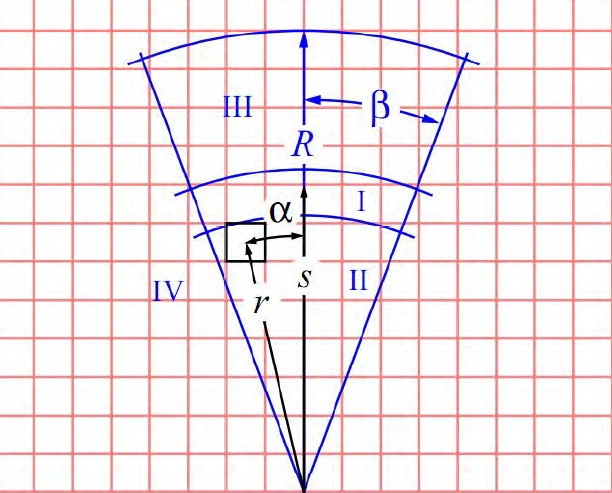
\includegraphics[scale = 0.35]{occ_grid_model.jpeg}
  \caption{Schema delle scansione}
  \label{fig:scan scheme}
\end{figure}

\noindent La regione I è la regione associata alla lettura effettiva del laser, la
regione II rappresenta un'area vuota in cui nulla viene rilevato, la regione III
è l'area coperta dal raggio laser, ma rimane sconosciuta se occupata o meno a
causa dell'occlusione, e la regione IV è al di fuori del campo di visibilità del \textsc{lidar}.
Parametri rilevanti della cella evidenziata (contorno nero) includono: $r$ che 
è la distanza dell'elemento di griglia dalla posizione del sensore; 
$\alpha$ l'angolo dell'elemento di griglia relativo al raggio centrale del sensore.
Per una misurazione $s$ che rientri nella regione I, la probabilità che la
misura sia effettivamente dovuta alla presenza di  un ostacolo in tale 
intervallo può essere calcolata dall'equazione (\ref{eq:lidargrid}):
%
\begin{equation}	
\label{eq:lidargrid}
P(s|Occupied) = \frac{\frac{R-r}{R} + \frac{ \beta- \alpha}{\beta} \beta}{2} 
\cdot Max_{\text{occupied}}
\end{equation}
%
dove $Max_{\text{occupied}}$, nell'eq.(\ref{eq:lidargrid}), è dovuto all'assunzione 
che una lettura di ``Occupato" non è mai completamente affidabile.
%A causa dell'occlusione, si assume che stato di occupazione nella regione III
%abbia il $50 \, \%$ di probabilità di essere occupato e/o il $50\,\%$
%di non essere occupato.
%
\subsection{Occupacy grid globale}
Ogni robot è dotato di memoria dove viene salvata la mappatura globale 
dell'intero ambiente. Questa, è definita occupacy grid globale, ed è ricostruita 
mediante rototraslazione e sovrapposizione delle occupacy grid locali 
fornite in diversi istanti dal robot.
Alla fine della simulazione le varie occupacy grid globali di ogni robot vengono
fuse in un'unica mappa.
Un problema per i metodi basati sulla griglia di occupazione è l'utilizzo della
memoria eccessivo, infatti diventa oneroso per la ricostruzione di mappe 3D. 
Un secondo problema è legato all'allineamento della griglia, assunto ideale, in
quanto è probabile che le celle: coprano aree difficili da raggiungere e zone 
parzialmente piene dove non è possibile catturare le acute discontinuità ai 
bordi degli oggetti. 

	
%Soluzione Proposta
\section{Soluzione Proposta}

	\subsection{Allocazione destinazioni ed Utility}
L'obiettivo di un processo di esplorazione è quello di coprire l'intero 
ambiente nel minor tempo possibile. Pertanto, è essenziale che i robot
tengono traccia di quali aree dell'ambiente sono già state esplorate. 
Inoltre, i robot devono costruire una mappa globale per pianificare i loro 
percorsi e coordinare le loro azioni.
Quando esploriamo un ambiente sconosciuto, siamo particolarmente 
interessati alle ``celle di frontiera". 
Con cella di frontiera, denotiamo ciascuna cella già esplorata che è un vicino
immediato di un cella sconosciuta, inesplorata. 
Se indirizziamo un robot a una tale cella, ci si può aspettare che ottenga 
informazioni sull'area inesplorata quando arriva alla sua posizione di 
destinazione.
Il fatto che una mappa in generale contiene diverse aree inesplorate solleva 
il problema di come assegnare in modo efficiente l'assegnazione delle 
destinazioni a più robot.
Se sono coinvolti più robot, vogliamo evitare che molti di loro si spostino 
nella stessa posizione. Per affrontare questi problemi e determinare i luoghi 
di destinazione appropriati per i singoli robot, il nostro sistema utilizza il 
seguente approccio: consideriamo contemporaneamente il costo del 
raggiungimento di una cella di frontiera e l'utilità di questa.
Per ogni robot, il costo per raggiungere la cella è proporzionale alla distanza 
tra se stesso e quest'ultima, d'altra parte l'utilità di una cella di frontiera dipende 
invece dal numero di robot che si stanno spostando in quella direzione o in 
posizioni limitrofe.\cite{burgard2005coordinated}
Di seguito vengono riportate le equazioni implementate:
\begin{equation}	
\label{eq:componet1}
U(t_n|t_1,\dots,t_{n-1} ) = U_{t_n} -  \sum_{i=1}^{n-1} P(||t_n - t_i ||)
\end{equation}

\begin{equation}	
\label{eq:componet2}
P(d) = \begin{cases} 
   1 - \frac{d}{maxrange}  	&  	\mbox{se } d < \text{maxrange} \\  
   0 									& 		\text{altrimenti}
   \end{cases}
\end{equation}

\begin{equation}	
\label{eq:componet3}
(i,t) = \text{argmax}_{i^{\iota},t^{\iota}} (U_{t^{\iota}}  -\beta V^{i^{\iota}}_{t^{\iota}} ) 
\end{equation}
%
La prime due equazioni (\ref{eq:componet1}--\ref{eq:componet2}), calcolano 
l'utility per il robot n-esimo mentre l'ultima equazione rappresenta il caso 
esteso all'integrazione di più robot che comunichino tra loro. 
\emph{Maxrange} rappresenta la massima visibilità fornita dal lidar, $d$ 
rappresenta la distanza dei target assegnati ai vari robot, $U$ la funzione di 
utility e $V$ la funzione di costo quest'ultima tiene conto della distanza di ogni 
robot dal suo target. Le $i$ e $t$, nell'eq.(\ref{eq:componet3}),  forniscono 
per ogni robot il suo target i-esimo ottimale.
Il modo in cui questi target da parte di ogni robot vengono raggiunti è 
lasciato alla funzione potenziale che verrà descritta in seguito.
	\subsection{Pianificazione}
\label{ssec:ArtPotField}
La pianificazione del percorso per i robot è uno dei criteri importanti da
prendere in considerazione per migliorare il livello di autonomia del robot.
Nella pianificazione del percorso, la sicurezza è un problema importante che 
dovrebbe essere preso in considerazione al fine di garantire che un robot 
raggiunga la posizione target senza collisioni con gli ostacoli circostanti.
Inoltre, ci sono aspetti importanti che devono essere affrontati nella 
pianificazione del percorso; tempo computazionale, percorso ottimale e 
completezza. 
Uno dei metodi più diffusi per la pianificazione dei percorsi è il metodo 
\emph{Campi Potenziali Artificiali}. 
Il metodo del potenziale è in grado di superare uno scenario sconosciuto, 
tenendo conto della realtà dell'ambiente corrente e del movimento del robot. 
Due tipi di forze sono coinvolte nel metodo del campo potenziale; forza attrattiva 
generata da obiettivi e forza repulsiva generata da ostacoli, di conseguenza, 
il robot deve riprogrammare un nuovo percorso\cite{apotetianfield}.
Utilizzando informazioni parziali sullo spazio di lavoro raccolte attraverso i 
sensori quindi le informazioni sensoriali sono integrate in una mappa secondo un 
paradigma \emph{sense---plan---move}.
Oppure utilizzare le informazioni sensoriali impiegate per pianificare moti 
secondo un paradigma \emph{stimulus---response} (navigazione reattiva).
Il robot è considerato come un punto sotto l'influenza dei campi prodotti da 
obiettivi e ostacoli nello spazio di ricerca. Le forze repulsive sono generate 
da ostacoli mentre la forza attrattiva è generata dagli obiettivi. La forza 
risultante (la somma di tutte le forze) dei campi sul robot viene utilizzato 
per determinare la direzione del movimento e la velocità di spostamento evitando 
collisioni\cite{5498220}.
Tuttavia esistono svantaggi quali:
\begin{enumerate*}[label={\alph*)},font={\bfseries}]
\item situazione di stallo dovuta ai minimi locali; 
\item oscillazione in presenza di ostacoli; 
\item nessun passaggio tra ostacoli ravvicinati; 
\item oscillazioni in passaggi stretti\cite{131810}.
\end{enumerate*}
Il robot viene considerato come punto $\mathbf{q} = (x \, y)^T$, in un piano 
cartesiano, attratto (potenziale $U_{\text{att}}$) dal punto obiettivo 
$\mathbf{q}_g$ e respinto (potenziale $U_{\text{rep}}$) dagli ostacoli.
\begin{equation}
\label{eq:apfm}
U(q) = U_{\text{att}}(q) + U_{\text{rep}}(q)
\end{equation}
%
\noindent dove $U(q)$ potenziale artificiale; $U_{\text{att}}(q)$ campo 
attrattivo; $U_{\text{rep}}(q)$ campo repulsivo.
La pianificazione avviene in modo incrementale: ad ogni configurazione 
$\mathbf{q}$, la forza artificiale viene generata come nell'equazione (\ref{eq:attractive}):
\begin{equation}
\label{eq:attractive}
\begin{split}
F(q) &= - \nabla U(q)\\
&= - \nabla U_{\text{att}}(q) -U_{\text{rep}}(q)\\
F(q) &= F_{\text{att}}(q) + F_{\text{rep}}(q)	
\end{split}
\end{equation}
dove $F(q)$: forza artificiale; $F_{\text{att}}(q)$: forza attrattiva; 
$F_{\text{rep}}(q)$: forza repulsiva. Il campo potenziale $U_{\text{att}}$) tra 
robot e obiettivo viene descritto da (\ref{eq:fieldattractive}) per trascinare 
il robot nell'area obiettivo.
\begin{equation}
\label{eq:fieldattractive}
\begin{split}
U_{\text{att}}(q) &= \frac{1}{2} \, k_a \, (q-q_d)^2\\
&= \frac{1}{2} \, k_a \, \rho^{2}_{goal}(q)
\end{split}
\end{equation}
dove $k_a$: coefficiente positivo per APF\footnote{Artificial Potential Field};
$q$: posizione corrente del robot; $q_{d}$: posizione corrente dell'obiettivo.
$\rho_{\text{goal}}(q) = \|q-q_{d}\|$ è una distanza euclidea dalla posizione 
del robot alla posizione dell'obiettivo. La forza attrattiva del robot è 
calcolata come gradiente negativo del potenziale campo\cite{6283526}:
\begin{equation}
\label{eq:gradientfield}
\begin{split}
F_{\text{att}}(q) &= -\frac{1}{2}k_a \rho^2_{\text{goal}}(q)\\
F_{\text{att}}(q) &= -k_a \, (q-q_d)
\end{split}
\end{equation}
%
$F_{\text{att}}(q)$, nell'eq. (\ref{eq:gradientfield}), è un vettore diretto 
verso $q_{\text{d}}$ con intensità linearmente proporzionale alla distanza da 
$q$ a $q_{\text{d}}$. Può essere scritto nelle sue componenti:
\begin{equation}
\label{eq:componet}
\begin{split}
F_{\text{att}} -x(q) &= -k_a \, (x - x_d)\\
F_{\text{att}} -y(q) &= -k_a \, (y - y_d)\\
\end{split}
\end{equation}
%
Le equazioni (\ref{eq:componet}) sono la forza attrattiva nelle direzioni $x$ 
e $y$. Nella funzione potenziale, il robot deve essere respinto dagli ostacoli, 
ma se lontano da questi, il movimento non risente della loro influenza.
La funzione potenziale di repulsione (\ref{eq:repulsive}) è:
\begin{equation}
\label{eq:repulsive}
U_{\text{rep}}(q) = 
\begin{cases} 
\frac{1}{2}k_b(\frac{1}{d(q)}-\frac{1}{d_0})^2 &\mbox{se } d(q) \leq d_0 \\ 
0 & \mbox{se } d(q) > d_0
\end{cases} 
\end{equation}
\begin{figure*}[htb]
\centering
\subfloat[][\emph{Campo attrattivo - repulsivo}.]
   {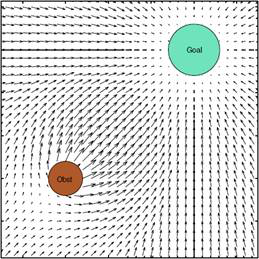
\includegraphics[width=.35\textwidth]{image008}} \quad
\subfloat[][\emph{Pianificazione traiettoria}.]
   {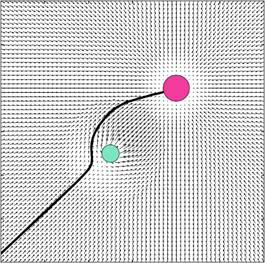
\includegraphics[width=.35\textwidth]{image010}} 
\caption{Potenziali artificiali}
\label{fig:potentialfield}
\end{figure*}

	\subsection{Algoritmi di stima}
Il sistema robotico preso in esame presenta degli errori all'ingresso degli
encoder, tale errore porta il sistema a manifestare nel lungo periodo il noto
comportamento di \emph{drift}.
Nasce allora il problema di correggere e stimare la posizione in base ad un dato
modello.
Stimando la posizione del robot utilizzando la ricostruzione odometrica si
ottiene un risultato affetto da incertezza crescente all'aumentare dello
spostamento.
È necessario quindi correggere tale stima attraverso il particle
filter\cite{newman2003} analizzato di seguito.
Ciò su cui ci appoggeremo per avere una stima della posizione assunta dal robot,
saranno dei sensori esterni ad esso, nel nostro caso delle ancore \textsc{Wi-Fi}
virtualmente simulate.

\subsubsection{Filtro Particellare}
L'algoritmo di localizzazione PF procede come segue in figura
\ref{fig:particle filter}. Si inizializzano $n$ particelle in una mappa.
Ogni particella è un vettore di stato $q\,=\,[x \, y \, \theta]^{T}$ del veicolo
ed ad ognuna di queste si applica il modello descritto dal sistema di eq.
(\ref{eq:modelcinematico}): e se ne aggiunge un rumore al vettore di
controllo $u\,=\,[v \, \omega]^{T}$.
Successivamente per ogni particella si prevede la possibile misura ottenibile e
si confronta con l'osservazione realmente effettuata dalla ancora
\textsc{Wi-Fi}, tale confronto porterà al calcolo dell'innovazione o di ciò che
definiremo peso della particella.
Si selezionano le particelle che meglio spiegano l'osservazione, un modo per
farlo è quello di costruire una pdf che descriva i campioni e i loro pesi, e
poi riselezionare un nuovo set di particelle da questa pdf.
La stima della posizione del robot fornita dal filtro è la media di questo
nuovo ricampionamento.
Il punto cruciale è che non richiede alcuna ipotesi di linearizzazione (non ci
sono jacobiani coinvolti) e non ci sono ipotesi Gaussiane. È particolarmente
adatto ai problemi con piccoli spazi di stato mentre in caso di vettori di
stato grandi diventa computazionalmente pesante.

\begin{figure}[!htb]
  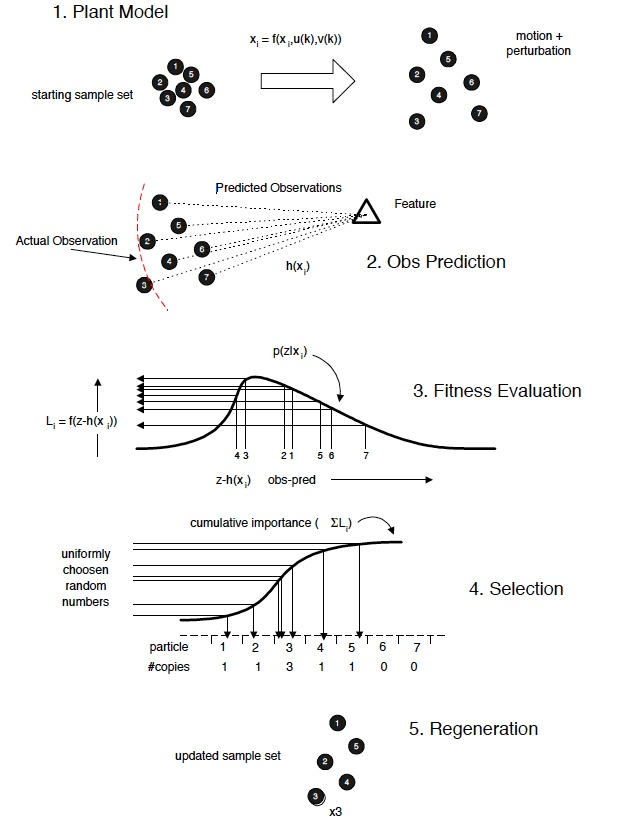
\includegraphics[scale = 0.4]{particle_filter}
  \caption{Filtro Particellare}
  \label{fig:particle filter}
\end{figure}


	
\section{Implementazione}
	\section{Implementazione}
\label{sec:implementazione}
Per la realizzazione del progetto si è optato per una simulazione con la suite
\textsc{matlab}, realizzando un software basato su un'architettura a oggetti
e funzionale per i motivi indicati di seguito.
\subsection{Esecuzione}
Una volta generato lo scenario la simulazione inizia con il posizionamento di
uno o più robot all'interno della mappa come condizione iniziale e assegnato un
obiettivo da raggiungere.
Questi non conosco l'ambiente in cui si trovano e quindi tentano di raggiungere
l'obiettivo nella maniera più rapida impostando un traiettoria rettilinea
determinata come norma tra due punti.
La pianificazione della traiettoria viene modificata in base alle rilevazioni
effettuate dal \textsc{lidar} in tal modo essi evitano l'ostacolo perché repulsi.
Per la creazione delle matrici di occupazione locali vengono utilizzate le misure
fornite dal lidar, tali misure vengono riproiettate nel sistema di riferimento del robot
e registrate all'interno di una matrice utilizzando come peso per ogni misura l'equazione
fornita da \eqref{eq:lidargrid}.
Queste verranno integrate in una matrice globale che sarà aggiornata ogni secondo. Il
passaggio da matrice locale a matrice globale avviene rototraslando rispetto la posizione
stimata del robot fornita dal particle filter e registrata all'interno del robot.La matrice
globale del robot si assume essere già dimensionata in base alla mappa da esplorare.
Il robot durante la sua esplorazione è programmato per affiancare il primo muro visibile e
percorrerlo,nel caso in cui durante questa operazione si dovessero presentare zone già visitate,
esso cercherà di raggiungere punti non ancora esplorati all'interno della stanza, questa operazione
viene condotta registrando le zone già esplorate dal robot all'interno di una seconda matrice assunta
anch'essa di una dimensione tale da permettere di contenere la stanza con la risoluzione voluta.
Il robot quando risulterà essere nel raggio di comunicazione con altri robot avvierà il meccanismo di Utility,
in base al quale sarà assegnato ad ogni robot comunicante un nuovo target da raggiungere che massimizzi
l'utilità, calcolata con la equazione \eqref{eq:componet3}. Per evitare la ricomunicazione tra robot è stato
inserito un delay che deve trascorrere tra una comunicazione e l'altra prima che i 2 robot possano ricomunicare
tra loro.La comunicazione come già detto risulta essere ideale senza degradazione di segnale.
Durante la comunicazione i robot condivideranno la mappa contenente le zone già visitate in modo da
non permettere il passaggio in zone già viste da altri robot.
%
\input{introOOP}
\subsection{Classe Map}
\label{ssec:ClassMap}
La classe Map gestisce la generazione di una nuova mappa di dimensioni variabili
o il caricamento di una precedentemente salvata. Nel costruttore è possibile
specificare come primo argomento se desidera una nuova mappa o una esistente
mediante stringa ``new" o ``load".
Fornendo come parametri in ingresso la dimensione della mappa desiderata.
Così si avvia il processo di generazione procedurale visto
nella sez. \ref{ssec:k-d}. Opzionalmente è possibile specificare se si
desiderano più punti di riferimento virtuali oltre quelli impostati di default.
Con la stringa ``load", invece è possibile richiamare una mappa esistente da
\textsc{gui}.
All'interno della classe sono salvati, come vettori, i punti che costituiscono
la mappa e le linee che li collegano. Questi sono interpretati dalla funziona
che simula il processo di scansione del \textsc{lidar}.
Per mappe di grandi dimensioni si estraggono i punti liberi che non siano
collegati a linee. Questo permette di fornire al robot le condizioni iniziali
all'avvio della simulazione evitando che venga posizionato all'interno di
qualche parete.

\subsection{Classe Robot}
\label{ssec:ClassRobot}
La classe Robot definita nel progetto permette di generare uno o più istanze di
questo oggetto permettendo così avere un comportamento univoco.
Tali istanze condividono le stesse proprietà non modificabili dall'esterno,
infatti sono messe a disposizione dell'utente metodi per l'accesso e la
modifica di queste.
Questo permette di avere robot che condividono, una volta configurati, gli
stessi parametri costanti i quali sono:
\begin{enumerate*}[label={\alph*)},font={\bfseries}]
	\item geometrici;
	\item risoluzione dei sensori;
	\item memoria di massa riservata per le scansioni;
	\item memoria di massa riservata per occupacy grid.
\end{enumerate*}
Tutti i paramenti salvati all'interno della classe sono accessibili in solo
lettura dall'esterno.
Infatti una volta create una o più istanze del robot queste sono posizionate
all'interno della mappa di cui non conoscono nulla se non quello che
percepiscono tramite \textsc{lidar} ogni 10 \si{\hertz}. Successivamente il
robot si muoverà in direzione delle coordinate obiettivo pianificando il
percorso di volta in volta secondo le informazioni ricevute dalla funzione
potenziali artificiali, vista precedentemente nella
sez. \ref{sec:soluzioneprop}.\ref{ssec:ArtPotField}.

\subsection{Classe Particle Filter}
\label{ssec:ClassPF}
La classe Particle Filter mette a disposizione due funzioni pubbliche:
\begin{enumerate*}[label={\alph*)},font={\bfseries}]
	\item il costruttore di classe;
	\item il metodo \emph{update}.
\end{enumerate*}
Il costruttore è utilizzato per generare
un'istanza di questo oggetto legata all'altra classe robot da cui riceve le
informazioni relative alle caratteristiche dei sensori e il vettore velocità.
Inoltre la classe riceve dall'altra classe Map, \ref{ssec:ClassMap}, le
posizioni dei punti di riferimento virtuali precedentemente generati.
Con il metodo \emph{update} invece viene aggiornata la stima della posizione del
robot ad ogni iterazione per la lunghezza della simulazione.

	

\section{Risultati}
\newpage

\section{Conclusioni}
\section{Conclusioni}
\label{sec:conclusioni}
È stato qui presentato un modo efficiente di condurre un'esplorazione coordinata
di un ambiente.
Possibile passo in avanti per la suddetta applicazione sarebbe la sua
realizzazione ed esecuzione fisica in modo da condurre uno studio più
approfondito sulle possibili problematiche riscontrabili.
Un limite evidente è la pianificazione di traiettorie come visto negli svantaggi
del metodo dei potenziali artificiali, nella sezione
(\ref{sec:soluzioneprop}.\ref{ssec:ArtPotField}), poiché viene perso molto tempo
nel modificare la traiettoria specialmente in prossimità degli ostacoli,
in sezioni di passaggio, e in ambienti ciechi.
Attualmente il robot si muove con velocità costante ponendo un freno allo spazio
esplorabile, un modello cinematico migliore permetterebbe lo studio del cambio
di velocità e accelerazione adattandole quando è necesario affrontare
deviazioni e in presenza o meno di ostacoli.
Inoltre si evidenzia che la generazione procedurale di mappe, vista nella
sezione (\ref{sec:soluzioneprop}.\ref{ssec:generazioneproc}), permette una
generazione di casistiche ampia, ma poco controllabile e incapace di riprodurre
strutture realmente esistenti nell'ambiente reale.
Una possibile evoluzione sarebbe la ricostruzione di uno scenario 3D.
Altro limite attuale dell'applicazione è il non riconoscimento di zone
inaccessibili, ciò comporta nel caso di zone inaccessibili molto estese una gran
probabilità di assegnazione di un target appartenente a tale zona per il robot.
Altri esempi di possibili migliorie software apportabili, sono: una migliore
rappresentazione fisica della comunicazione, robot-robot e robot-ancora
\textsc{Wi-Fi}, tramite gli ultimi protocolli esistenti e l'adozione di algoritmi
per una stima distribuita della posizione (least-square o di kalman distribuito).
	


	
%	\input{Result}
\newpage
%----------------------------------------------------------------------------------------
%	Bibliography
%----------------------------------------------------------------------------------------
	\clearpage
	\bibliographystyle{IEEEtran}
	\bibliography{bibliografia.bib}
\end{document}